\section*{Цель работы}

\begin{enumerate}
    \item Изучение входной ВАХ и семейства выходных ВАХ биполярного 
    транзистора в схеме включения с общим эмиттером;
    \item Расчёт усилительного каскада с общим эмиттером с заданием
    рабочей точки транзистора с помощью отрицательной
    обратной связи по току;
    \item Исследование усилительного каскада с общим эмиттером.
\end{enumerate}



\section*{Исходные данные}

Все исследования, проводимые в лабораторной работе, выполняются с 
биполярным транзистором 2N4401 согласно 16 варианту.
Из технических характеристик транзистора
\begin{itemize}
    \item максимальный ток коллектора $I_{K_{max}}=600mAdc$;
    \item максимальное напряжение коллектор-эмиттер $U_\text{КЭ$_{max}$}=40Vdc$;
    \item коэффициент усиления по току $h_{FE}=20..300$;
    \item максимальная рассеиваемая мощность $P_{D_{max}}=625mW$.
\end{itemize}


\section*{Снятие входной ВАХ биполярного транзистора}

Для снятия входной ВАХ биполярного транзистора в
программной среде LTspice будем использовать источник тока,
который формирует максимальный ток 
$$
I_\text{Б}=\frac{I_{K_{max}}}{h_{FE}}=\frac{0.6A}{160}=3.75mA.
$$

Результат снятия входной ВАХ биполярного транзистора со схемы на
рисунке \ref{fig:схемавах} показано на рисунке \ref{fig:длявах} с двумя
графиками для $U_\text{KЭ}=0V$ и $U_\text{KЭ}=5V$.
По графику с курсорами (см. Рис \ref{fig:h11}) определили $\Delta U_\text{БЭ}=62.00\ mV$, $\Delta I_\text{Б}=2.42\ mA$ и нашли
\begin{equation*}
    h_{11}=\frac{\Delta U_\text{БЭ}}{\Delta I_\text{Б}}=\frac{62.00\ mV}{2.42\ mA}=25.61\ \Omega.
\end{equation*}
По графику с курсорами (см. Рис \ref{fig:h12}) определили $\Delta U_\text{БЭ}=155.69\ mV$; $\Delta U_\text{КЭ}=5\ V$ и нашли
\begin{equation*}
    h_{12}=\frac{\Delta U_\text{БЭ}}{\Delta U_\text{КЭ}}=\frac{155.69\ mV}{5\ V}=0.03\ .
\end{equation*}


\begin{figure}[H]
    \centering
    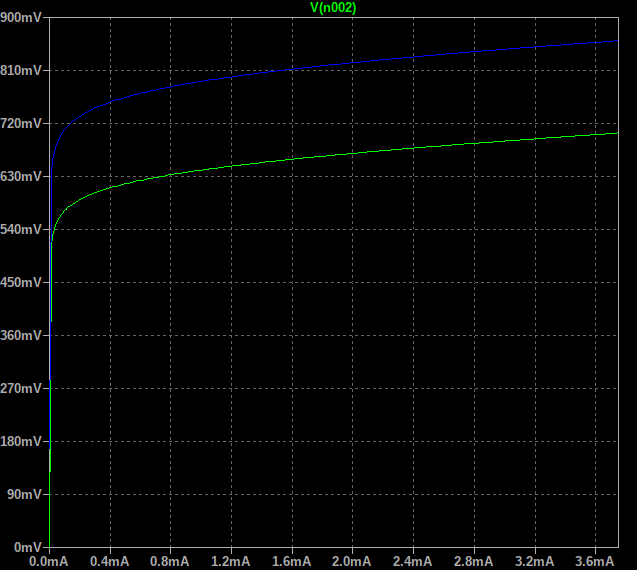
\includegraphics[width=0.8\textwidth]{figs/длявах.png}
    \caption{Входная ВАХ биполярного транзистора}
    \label{fig:длявах}
\end{figure}

\begin{figure}[H]
    \centering
    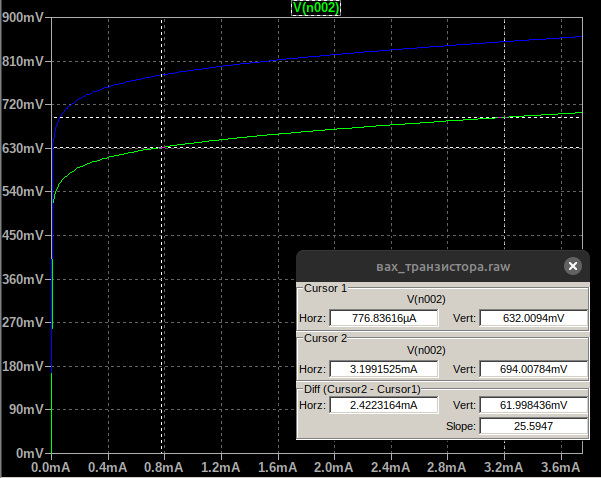
\includegraphics[width=0.8\textwidth]{figs/h11.png}
    \caption{Входная ВАХ биполярного транзистора с курсорами для нахождения $h_{11}$}
    \label{fig:h11}
\end{figure}

\begin{figure}[H]
    \centering
    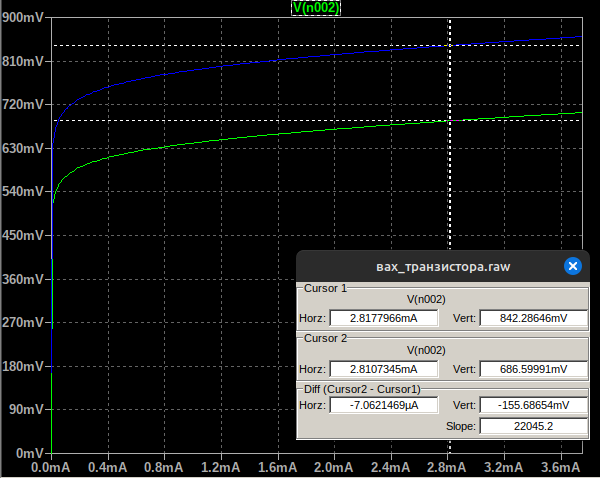
\includegraphics[width=0.8\textwidth]{figs/h12.png}
    \caption{Входная ВАХ биполярного транзистора с курсорами для нахождения $h_{12}$}
    \label{fig:h12}
\end{figure}

\begin{figure}[H]
    \centering
    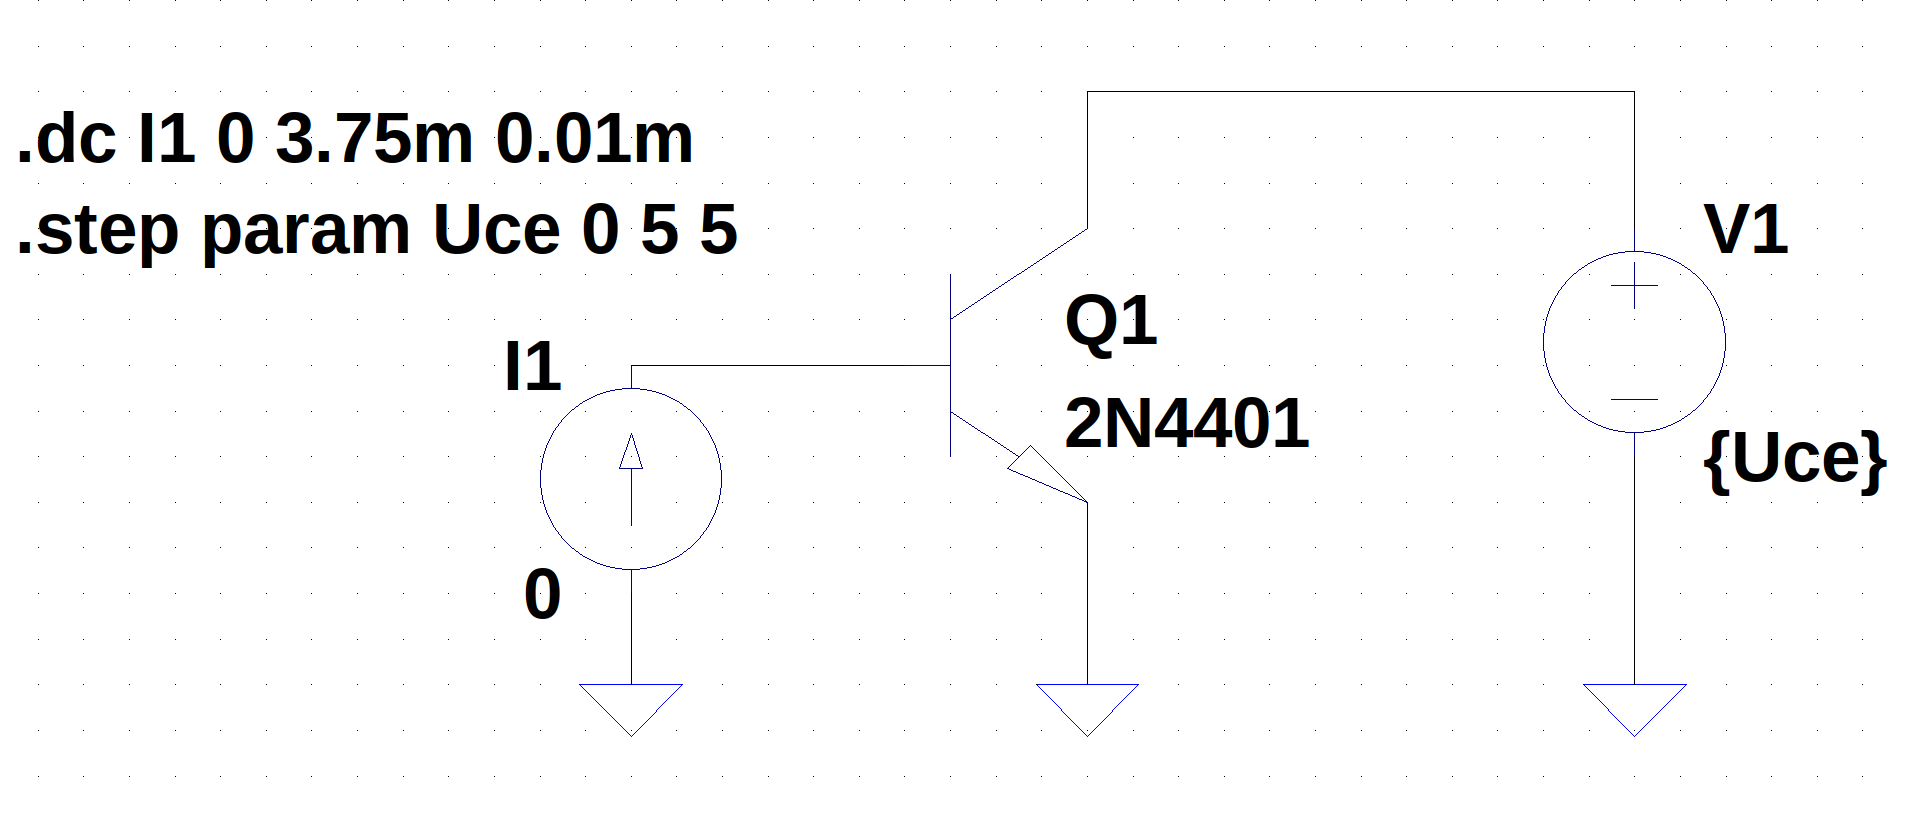
\includegraphics[width=1\textwidth]{figs/схемавах.png}
    \caption{Схема входной снятия ВАХ биполярного транзистора}
    \label{fig:схемавах}
\end{figure}



\section*{Снятие выходной ВАХ биполярного транзистора}

Для снятия выходной ВАХ воспользуемся схемой с рисунка \ref{fig:схемавахдлявыхода}.
Результат снятия выходной ВАХ биполярного транзистора можно увидеть на рисунке \ref{fig:выходвах},
на нем несколько графиков ВАХ для разных сил токов базы. 
По рисунку \ref{fig:h21} можно определить $\Delta I_K=51.97\ mA$, a так как графики соответствовали
токам базы $1.450\ mA$, $1.825\ mA$ $\Delta I_\text{Б}=0.375\ mA$, тогда
\begin{equation*}
    h_{21}=\frac{\Delta I_K}{\Delta I_\text{Б}}=\frac{51.97\ mA}{0.375\ mA}=138.59\ .
\end{equation*}\ 
По рисунку \ref{fig:h22} определим величины
$\Delta I_K=38.043\ mA$, $\Delta U_\text{КЭ}=10.171\ V$, тогда
\begin{equation*}
    h_{22}=\frac{\Delta I_K}{\Delta U_\text{КЭ}}=\frac{38.043\ mA}{10.171\ V}=0.004\ \frac{1}{\Omega}.
\end{equation*}

\begin{figure}[H]
    \centering
    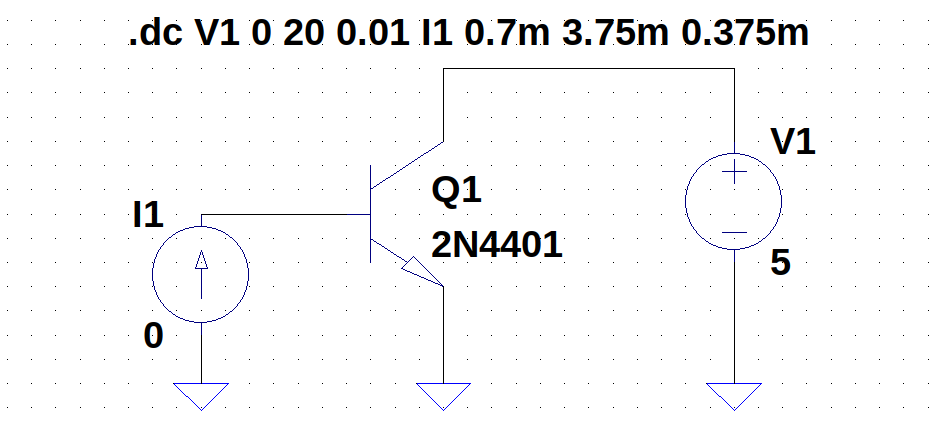
\includegraphics[width=1\textwidth]{figs/схемавахдлявыхода.png}
    \caption{Схема выходного снятия ВАХ биполярного транзистора}
    \label{fig:схемавахдлявыхода}
\end{figure}

\begin{figure}[H]
    \centering
    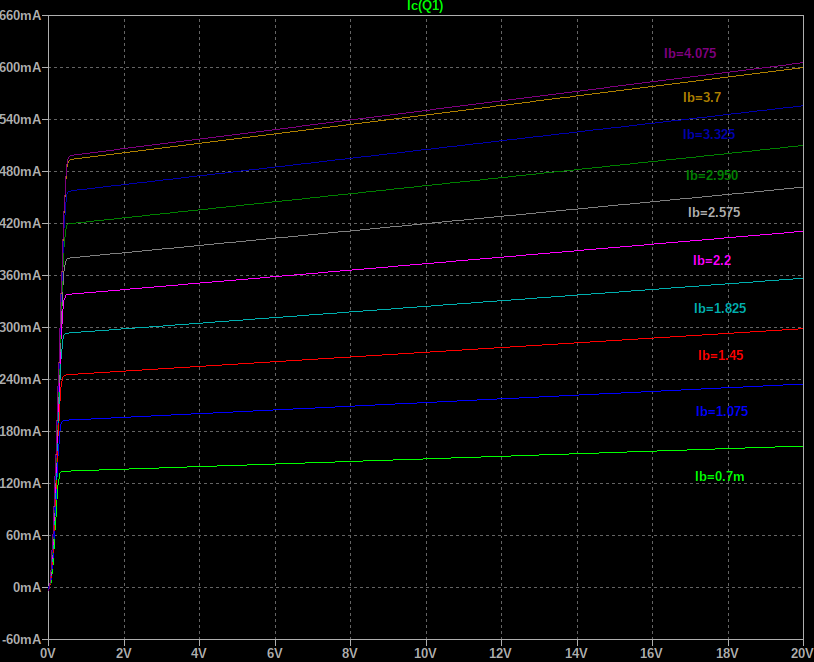
\includegraphics[width=0.8\textwidth]{figs/выходвах.png}
    \caption{Выходная ВАХ биполярного транзистора}
    \label{fig:выходвах}
\end{figure}

\begin{figure}[H]
    \centering
    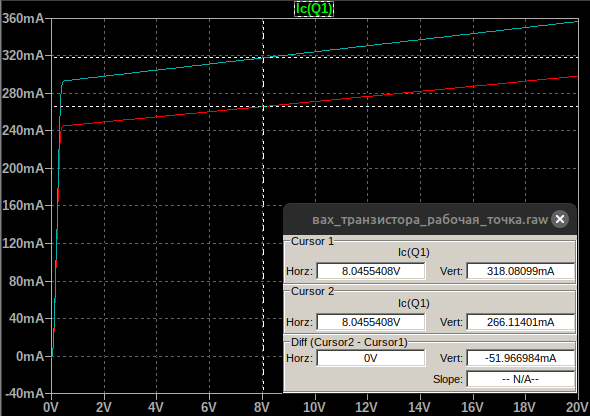
\includegraphics[width=0.8\textwidth]{figs/h21.png}
    \caption{Выходная ВАХ биполярного транзистора с курсорами для нахождения $h_{21}$}
    \label{fig:h21}
\end{figure}

\begin{figure}[H]
    \centering
    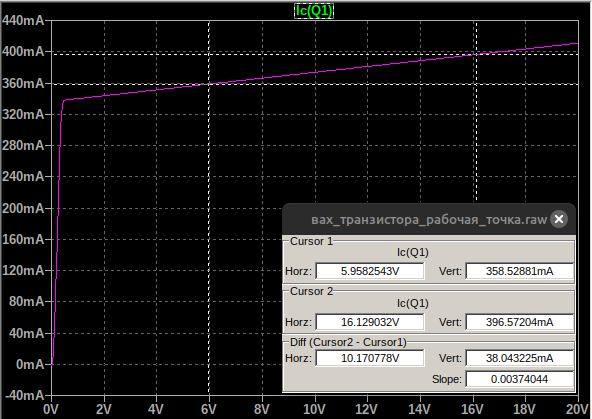
\includegraphics[width=0.8\textwidth]{figs/h22.png}
    \caption{Выходная ВАХ биполярного транзистора с курсорами для нахождения $h_{22}$}
    \label{fig:h22}
\end{figure}

Таким образом входное и выходное сопротивления транзистора
$R_{\text{ВХ}_{VT}}=h_{11}=25.61\ \Omega$ и $R_{\text{ВЫХ}_{VT}}=\frac{1}{h_{22}}=250\ \Omega$,
соответственно, коэффициент передачи по току транзистора $\beta=h_{21}=138.59$, что соответствует
техническим характеристикам транзистора.




\section*{Задание рабочей точки с помощью отрицательной
обратной связи по току}

На выходной ВАХ строим линию максимальной мощности $P_{D_{max}}=U_\text{КЭ}I_\text{К}=const$,
из даташита $P_{D_{max}}=625\ mW$, так значение силы тока будет ограничиваться максимальным
током коллектора $I_{K_{max}}=600\ mAdc$, а максимальное напряжение коллектора - $U_\text{КЭ$_{max}$}=40\ Vdc$.

Выберем значение напряжения источника питания $E_K=0.5U_\text{КЭ$_{max}$}=20\ V$.
Из условия передачи максимальной мощности от источника
энергии к потребителю выберем $R_K=160\ \Omega$, а 
$R_\text{Э}=5\ \Omega$. 
\begin{equation*}
    U_\text{КЭ}=E_K\Big|_{I_K=0}=20V\Big|_{I_K=0},
\end{equation*}
\begin{equation*}
    I_K=\frac{E_K}{R_K+R_\text{Э}}\Big|_{U_\text{КЭ}=0}=121\ mA\Big|_{U_\text{КЭ}=0}.
\end{equation*}
Тогда линию нагрузки будет выглядеть как рисунке \ref{fig:линии}.
\begin{figure}[H]
    \centering
    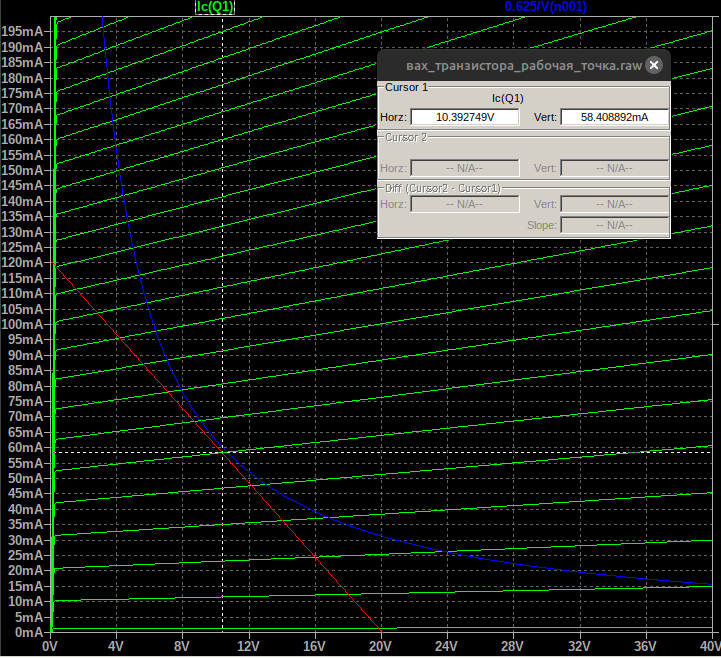
\includegraphics[width=1\textwidth]{figs/линии.png}
    \caption{Выходная ВАХ биполярного транзистора с линиями максимальной мощности (синяя) и нагрузки (красная)}
    \label{fig:линии}
\end{figure}

Зададим рабочую точку в середине нагрузочной линии. Для нее с помощью курсора
определим $I_{K_0}=58.41\ mA$, $U_{\text{КЭ}_0}=10.39\ V$ и $I_{\text{Б}_0}=0.26\ mA$ - значение
тока базы выбранное по соответствующей кривой выходной ВАХ, проходящей через
точку покоя. Напряжение $U_{\text{БЭ}_0}$ находится по входной ВАХ для ранее 
выборанного значения тока базы $I_{\text{Б}_0}$, следственно согласно рисунку \ref{fig:вахвходноедлярабточки}
$U_{\text{БЭ}_0}=741.47\ mV$.
\begin{figure}[H]
    \centering
    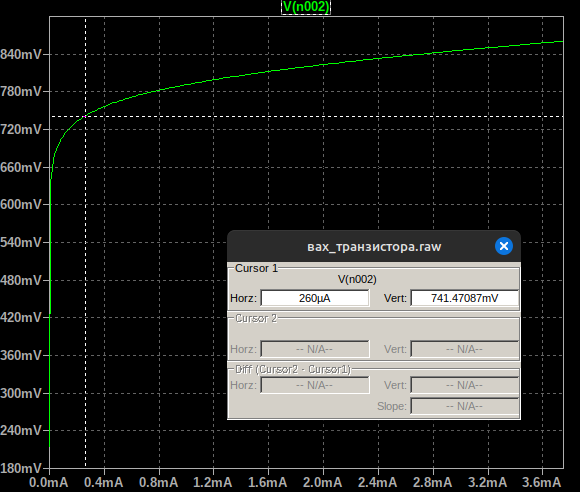
\includegraphics[width=0.8\textwidth]{figs/вахвходноедлярабточки.png}
    \caption{Входная ВАХ биполярного транзистора с курсором для нахождения $U_{\text{БЭ}_0}$}
    \label{fig:вахвходноедлярабточки}
\end{figure}

Зададим ток делителя $I_\text{Д}=5I_{\text{Б}_0}=1.3\ mA$, таким образом $I_{R_1}=I_\text{Д}=1.3\ mA$.
Зная ток, текущий через резистор $R_1$, можно найти значение его сопротивления
\begin{equation*}
    R_1=\frac{E_K-U_{\text{БЭ}_0}-U_{R_\text{Э}}}{I_{R_1}},
\end{equation*}
где $U_{R_\text{Э}}=(I_{K_0} + I_{\text{Б}_0})R_\text{Э}=E_K-I_{K_0}R_K-U_{\text{КЭ}_0}=20V-0.05841A\cdot 160\Omega-10.39V=0.2644V$,
\begin{equation*}
    R_1=\frac{20V-0.74147V-0.2644V}{0.0013A}=14,610\ \Omega= 14.61\ k\Omega.
\end{equation*}
Далее находим значение сопротивления резистора
\begin{equation*}
    R_2=\frac{U_{\text{БЭ}_0}+U_{R_\text{Э}}}{I_{R_1}-I_{\text{Б}_0}}=\frac{0.74147V+0.2644V}{0.0013A-0.00026A}\approx 967\ \Omega.
\end{equation*}

Рассчитаем значение емкостей конденсаторов. Рассчитаем значение емкостей конденсаторов.
Для расчета емкости конденсаторов можно воспользоваться соотношениями
\begin{equation*}
    C_\text{Э}=\frac{10\dots50}{2\pi f_\text{Н}R_\text{Э}}=\frac{30}{2\pi\cdot1000\cdot 5}=9.55E-4,
\end{equation*}
\begin{equation*}
    C_1=\frac{10\dots50}{2\pi f_\text{Н}R_\text{ВХ}}=\frac{30}{2\pi\cdot1000\cdot 25.61}=1.86E-4,
\end{equation*}
\begin{equation*}
    C_2=\frac{10\dots50}{2\pi f_\text{Н}R_\text{Н}}=\frac{30}{2\pi\cdot1000\cdot 25.61}=1.86E-4,
\end{equation*}
при расчете $C_2$ предположили, что нагрузкой является аналогичный каскад, т.о. $R_\text{Н}=R_\text{ВХ}$.

Соберем в LTspice схему усилителя на биполярном транзисторе, включенного по схеме с общим эмиттером,
ее можно увидеть на рисунке \ref{fig:каскад}. Параметры элементов заданы в соответствии с расчетом, 
проведенным ранее.
\begin{figure}[H]
    \centering
    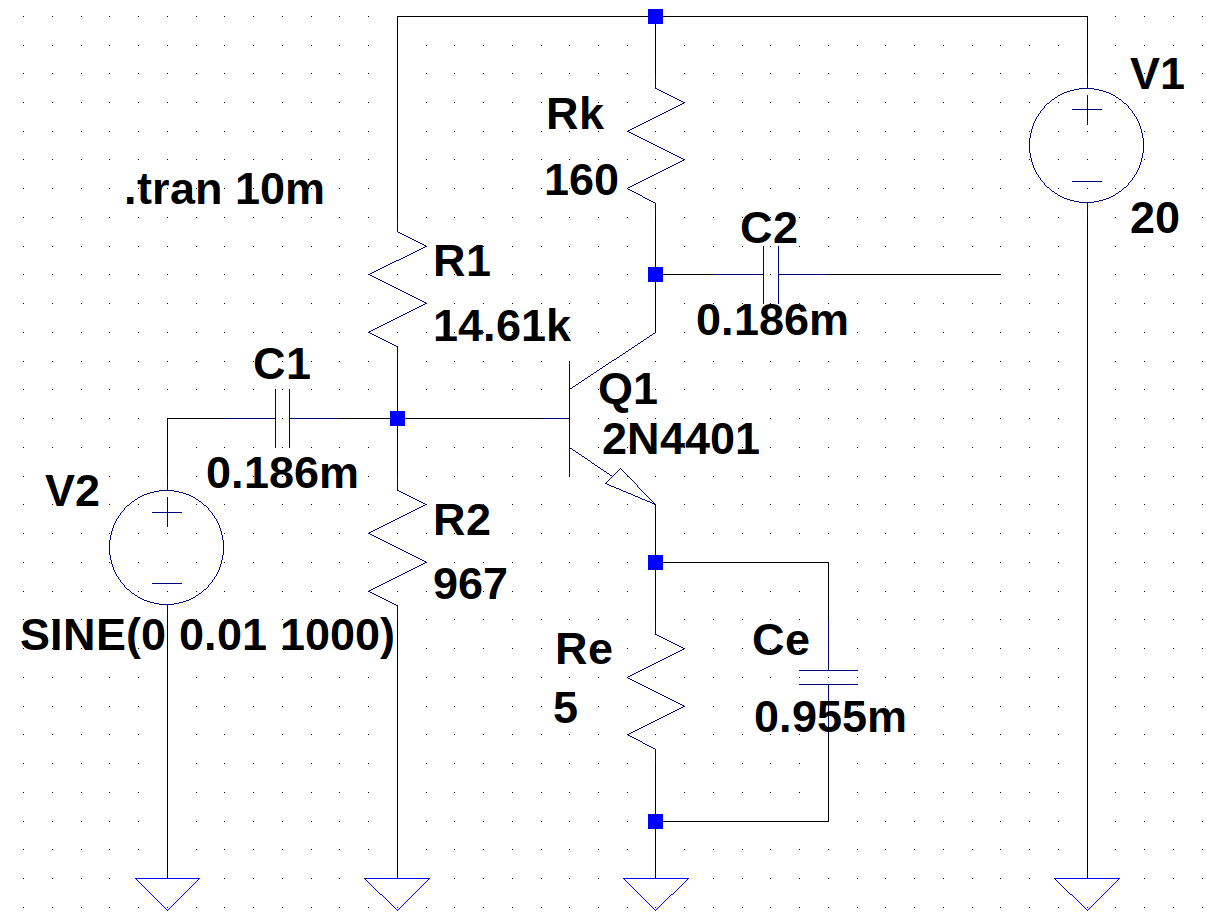
\includegraphics[width=0.8\textwidth]{figs/каскад.png}
    \caption{Схема усилителя на биполярном транзисторе}
    \label{fig:каскад}
\end{figure}
Проверим соответствие полученной точки покоя расчетным значениям. Для этого произведем 
моделирование работы схемы при отсутствии входного сигнала. Были сняты
$I_K=55.49mA,\ I_\text{Б}=0.25mA,\ U_\text{КЭ}=10.84V,\ U_\text{БЭ}=739.60mV$,
для сравнения $I_{K_0}=58.41mA,\ I_{\text{Б}_0}=0.26mA,\ U_{\text{КЭ}_0}=10.39V,\ U_{\text{БЭ}_0}=741.47mV$,
значения крайне близки.

Проведем моделирование схемы при гармоническом входном сигнале с частотой $1kHz$,
графики входных и выходных напряжений и сил токов можно увидеть на рисунках
\ref{fig:энднапряжения} и \ref{fig:эндток}. Как и ожидается от схемы подключения
транзистора с общим эммитером, напряжение и ток усиливаются. Рассчитаем
коэффициенты усиления по напряжению и току:
\begin{equation*}
    K_I=\frac{29.03mA}{0.14mA}=207\approx\beta=139,
\end{equation*}
\begin{equation*}
    K_U=\frac{2.21V}{0.01V}=221\approx\beta\frac{R_K}{R_\text{ВХ}}=139\cdot\frac{160}{25.61}=868.
\end{equation*}
Коэффициент усиления по мощности $K_P$:
\begin{equation*}
    K_P=K_IK_U=120652.
\end{equation*}

\begin{figure}[H]
    \centering
    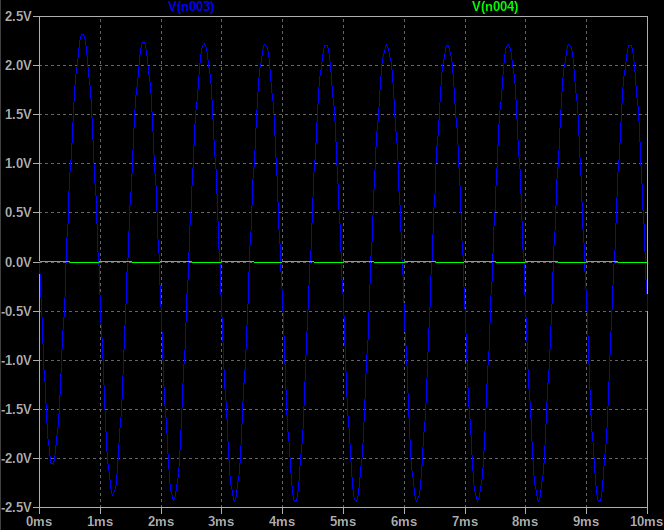
\includegraphics[width=0.8\textwidth]{figs/энднапряжения.png}
    \caption{График входного (зеленое) и выходного (синее) напряжений моделирования схемы при гармоническом входном сигнале}
    \label{fig:энднапряжения}
\end{figure}
\begin{figure}[H]
    \centering
    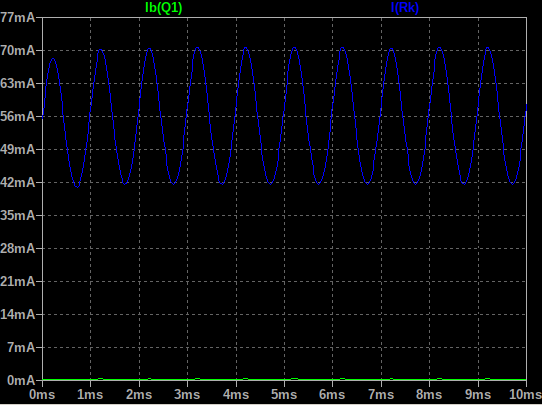
\includegraphics[width=0.8\textwidth]{figs/эндток.png}
    \caption{График силы тока базы (зеленое) и коллектора (синее) моделирования схемы при гармоническом входном сигнале}
    \label{fig:эндток}
\end{figure}

Проведем частотный анализ схемы с помощью режима \textit{AC analysis}. Полученную характеристику
можно увидеть в рисунке \ref{fig:ачх}. На нем сплошной линией обозначена амплитуда, а пунктиром - фаза.
\begin{figure}[H]
    \centering
    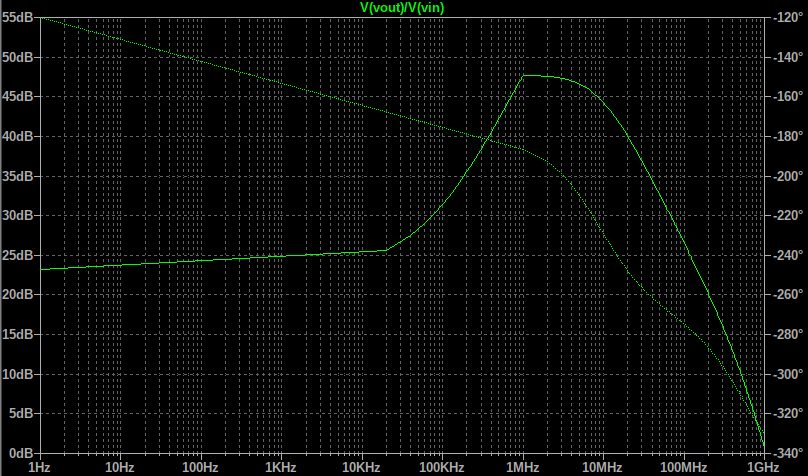
\includegraphics[width=1\textwidth]{figs/ачх.png}
    \caption{АЧХ коэффициента усиления схему по напряжению}
    \label{fig:ачх}
\end{figure}

\section*{Выводы}

В ходе лабораторной исследовали входные и выходные ВАХ биполярного
транзистора 2N4401, а также рассмотрели одно из его применений, а именно транзистор как
усилитель в схеме с общим эммитером. Для оценки усиления использовался коэффициент усиления тока, 
напряжения и мощности.


